%*******************************************************************
% Kapitel 2
%*******************************************************
\chapter{Approach}
\label{ch:Approach}

\section{Selecting a Web Development Stack}

As it was clear that we have to develop a web application we had to decide on the web development stack that we want to use. It was decided to split the team of four into pairs of two so that one pair does frontend development and the other pair does backend development. This decision allowed for each pair to choose the technologies they felt comfortable with which in turn improves development of the whole application.

In regards of frontend development it was intuitive to choose a JavaScript/Node.js stack as it is the primary programming language used for web development in general. The framework or library of choice was React. React is one of the most-used frontend technologies besides Angular and Vue.js. Its ecosystem is huge and comes with lots of reusable components and other libraries one can get from npm, e.g. reusable components for our \acs{CSS} framework of choice Bulma.

\begin{figure}[bth]
    \centering
    
\includegraphics[width=0.8\textwidth]{Graphics/Chapter2/frontend-backend-stack.png}
    \caption{Key technologies used for frontend \& backend}
\end{figure}

On the backend side it was decided to use Java and the Spring Framework. Reason being that the Spring Framework ecosystem provides a lot of useful projects and dependencies one can use. For example, Spring comes with abstractions for connecting to a database (Spring Data) or handling OAuth authentication (Spring Security). It was also decided to leverage the new, reactive stack of Spring called WebFlux. Using WebFlux we can make sure that the backend application is fast and responsive which in turn makes it behave similar to a Node application as well.

Choosing a database technology to accompany the backend application was fairly easy. Using Spring we basically could decide between PostgreSQL, MS SQL and MySQL/MariaDB as those databases are the only ones that are supported by the reactive stack at the time of writing (excluding H2 which we have used as an in-memory database mostly during the beginning of development). Even though we probably would have been able to use MS SQL we did not see the need to. As we have done previous projects using PostgreSQL we knew that it is easy to install on Linux and that we could also install pgAdmin to manage the database through an \ac{UI}.

\begin{figure}[bth]
    \centering
    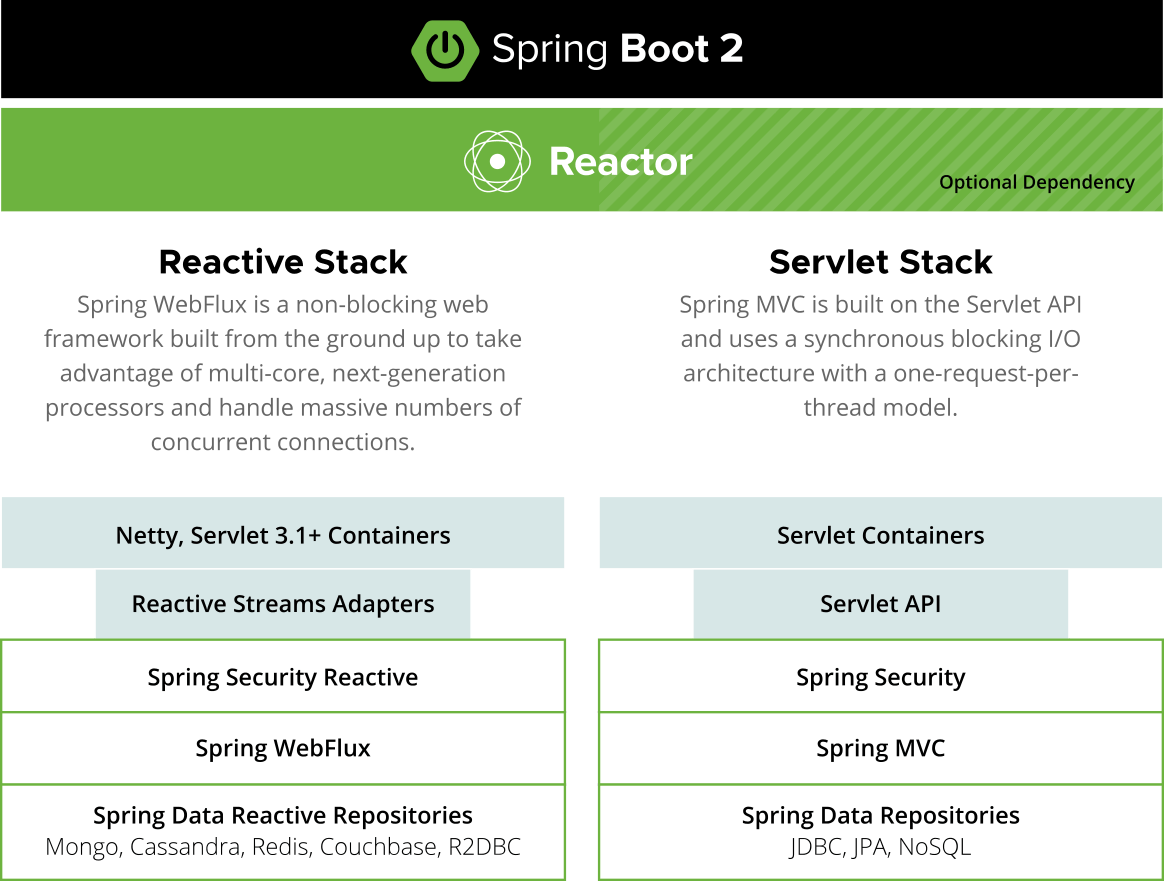
\includegraphics[width=0.9\textwidth]{Graphics/Chapter2/spring-stack.png}
    \caption{Overview of the reactive Spring stack \cite{SpringReactive}}
\end{figure}

\section{Using the Spotify API}

Looking at the Spotify Million Playlist Dataset one quickly will notice that it does not contain that much track, album and artist information.

\begin{lstlisting}[caption={Excerpt of one track entry in the Spotify Million Playlist Dataset}, style=Terminal]
{
    "pos": 0,
    "artist_name": "Missy Elliott",
    "track_uri": "spotify:track:0UaMYEvWZi0ZqiDOoHU3YI",
    "artist_uri": "spotify:artist:2wIVse2owClT7go1WT98tk",
    "track_name": "Lose Control (feat. Ciara & Fat Man Scoop)",
    "album_uri": "spotify:album:6vV5UrXcfyQD1wu4Qo2I9K",
    "duration_ms": 226863,
    "album_name": "The Cookbook"
}
\end{lstlisting}

Not only is the dataset missing information that we would like to use, e.g. links to the cover art, but it also does provide incomplete data, e.g. \texttt{artist\_name} missing artists in case of multiple artists, and data that we do not need anyway, e.g. \texttt{duration\_ms}. Luckily it contains all key information that we need to query Spotify for the data that we need. We can make use of the Spotify URIs which each have their API endpoint to query information for. Note that only the complete \ac{URI} is unique and that we absolutely need the prefix to the 22 character identifier. For more details, see \href{https://boonepeter.github.io/posts/2020-11-10-spotify-codes/}{\textit{How do Spotify Codes work?} by Peter Boone}.

Additionally, we use the Spotify Web API to authenticate users using OAuth 2.0. This is really useful as we do not have to implement our own authentication but just can use existing and secure OAuth through a client implementation. It also does provide us with user information such as their name and avatar. We can use this information to personalize the application and experience for the user. Finally, using the provided OAuth server we also can ask for specific scopes the user has to explicitly grant to our application, e.g. when reading a user's recently played tracks or other personal data.

\begin{figure}[bth]
    \centering
    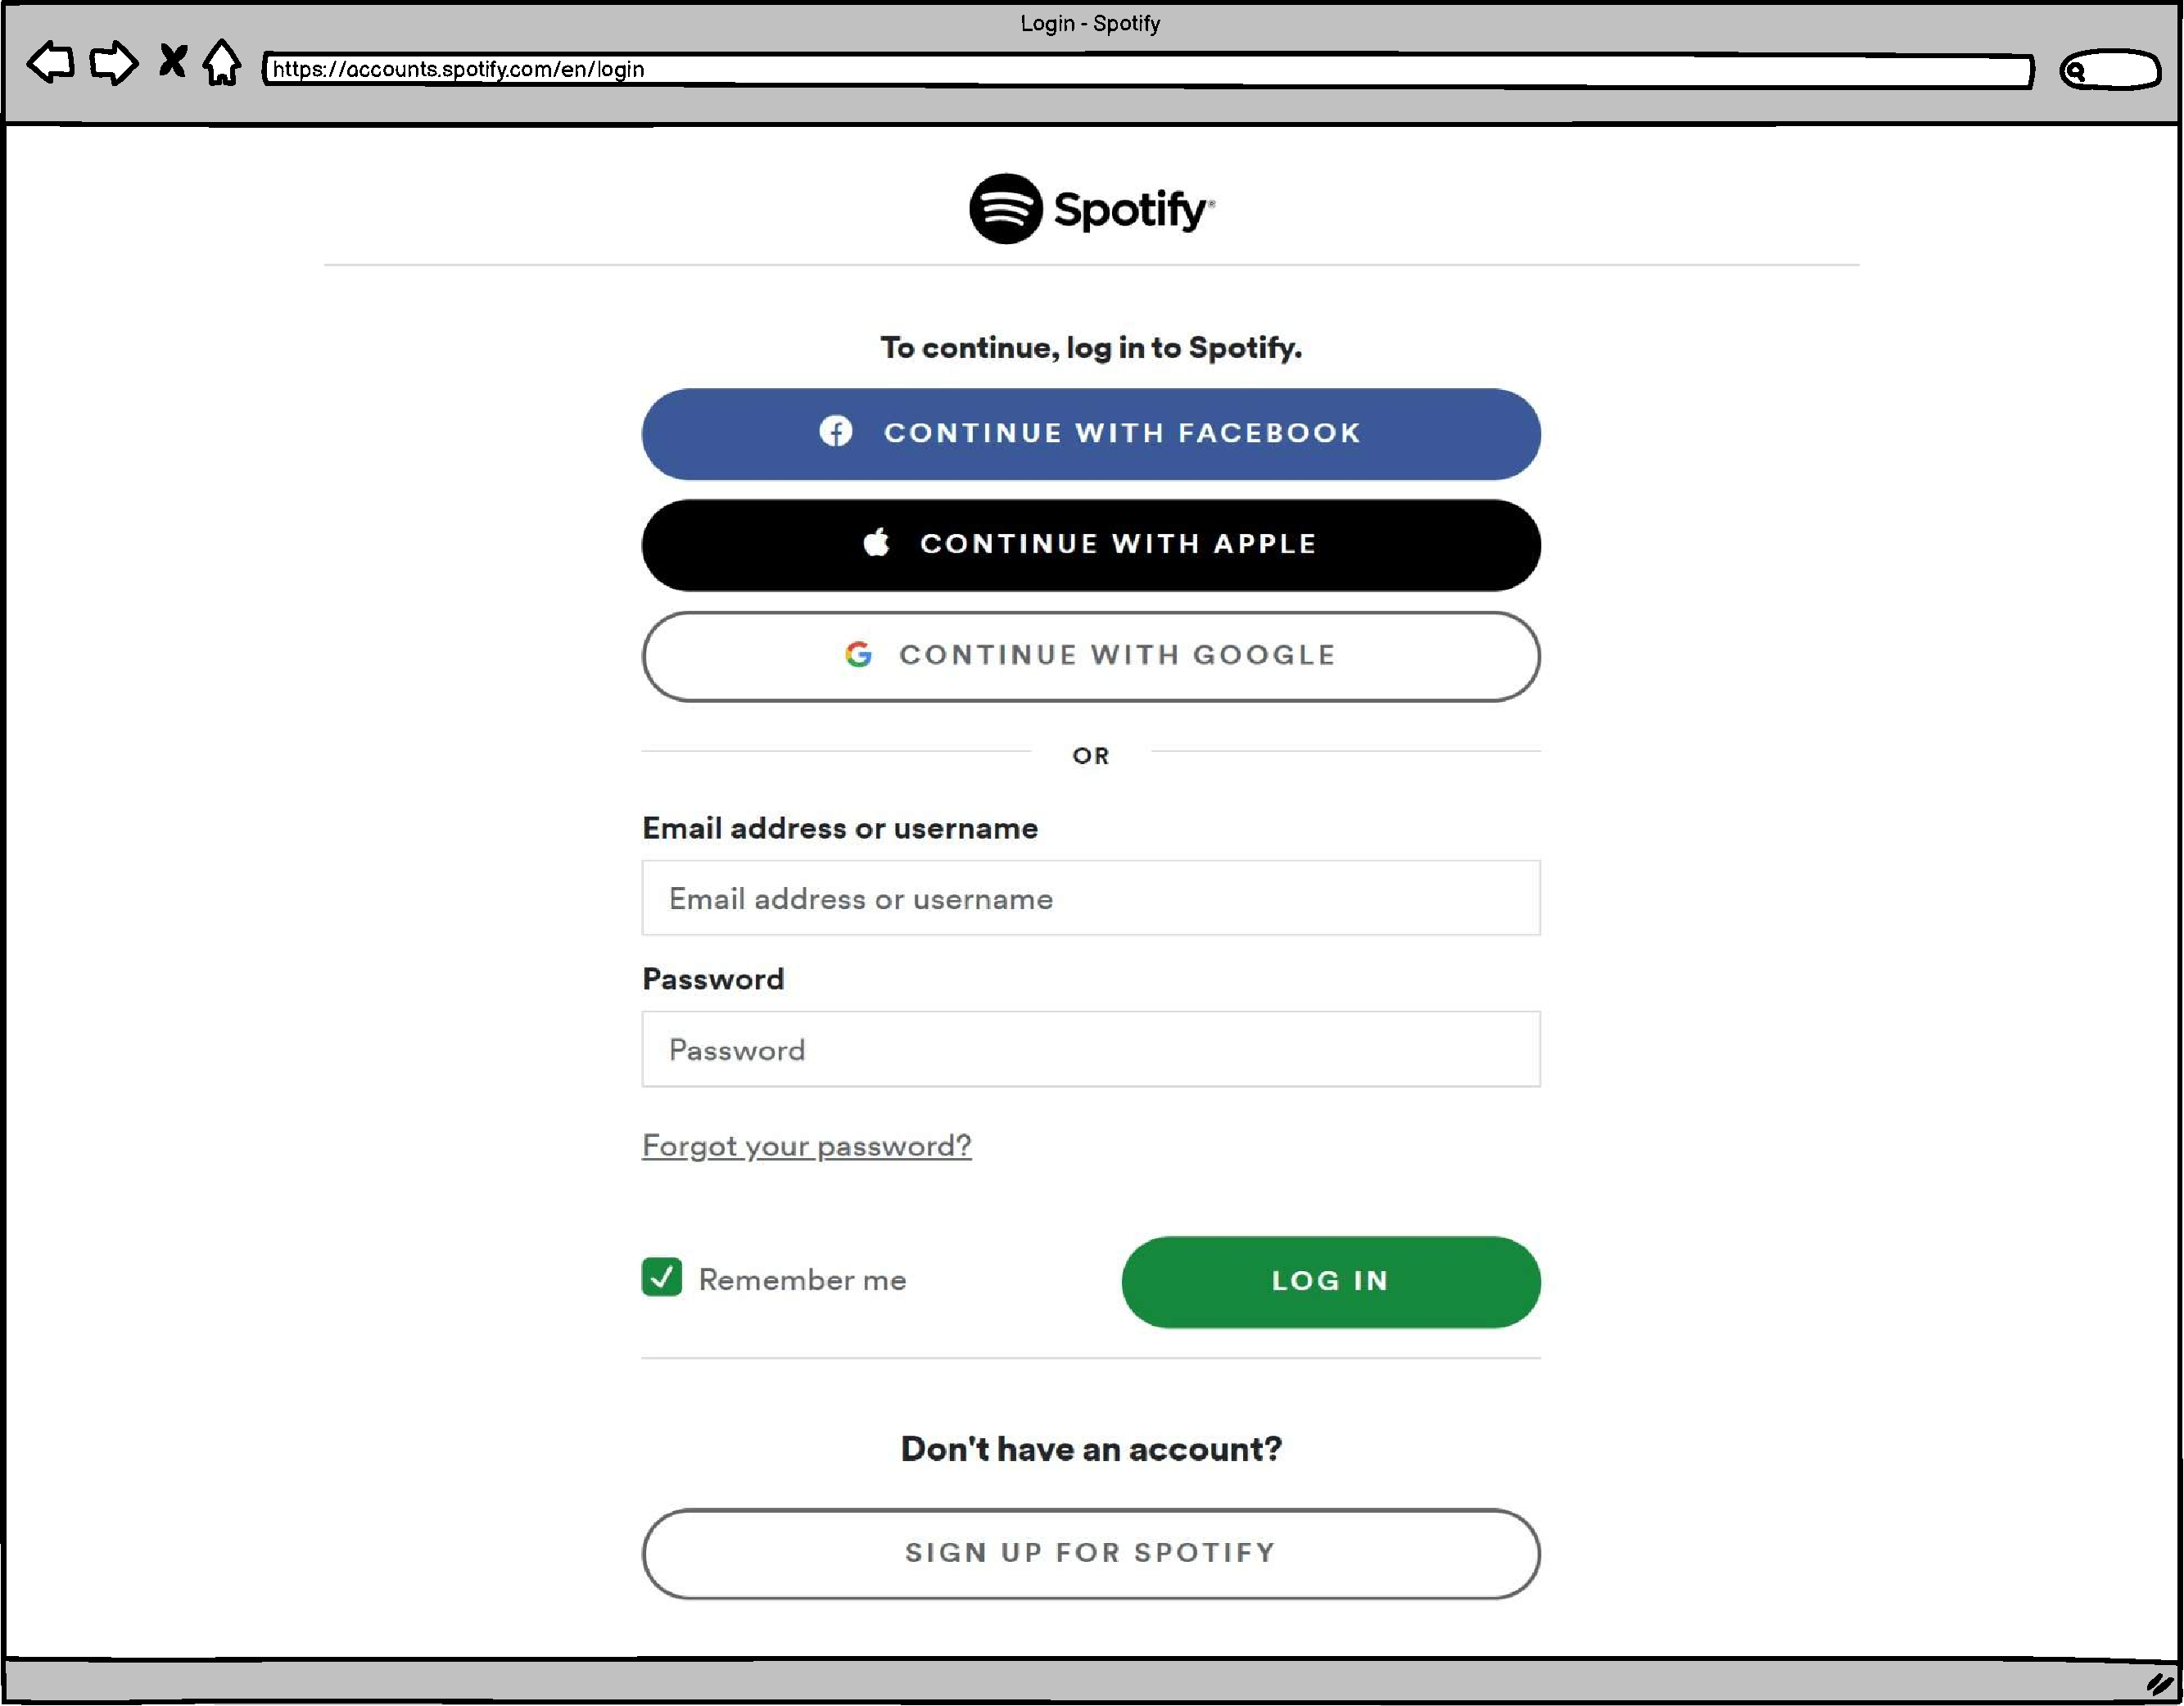
\includegraphics[width=1.0\textwidth]{Graphics/Chapter2/spotify-login.pdf}
    \caption{Spotify login dialog handling authentication with the application}
    \label{fig:SpotifyLogin}
\end{figure}

\section{Deciding on the Recommendation Algorithm}

In the beginning there was this idea to learn embeddings for tracks, albums and artists. We did consider using the Word2Vec implementation in Deeplearning4j but discarded the idea quickly as no team member has ever used that library before and we decided that trying to use that implementation would most likely take too much time. Instead we have decided that simply calculating similarities between two sets of tracks would be a good starting point and that the application could then still be extended in case the results of the recommender system would have been unsatisfactory.

We would then choose the Jaccard similarity to compute similarities between two sets of tracks with one of those sets being a playlist the user provides and the other one being a playlist form the Spotify Million Playlist Dataset. The Jaccard similarity would then compute the similarity by dividing the intersection of both sets with their union yielding a number between 0 and 1.

\begin{equation}
    J(A,B) = {{|A \cap B|}\over{|A \cup B|}} = {{|A \cap B|}\over{|A| + |B| - |A \cap B|}}
\end{equation}

\begin{lstlisting}[caption={Jaccard implementation as a \acs{SQL} function in PostgreSQL}, style=Base, language=SQL]
CREATE FUNCTION my_jaccard(VARIADIC track_uris varchar[])
RETURNS TABLE(jaccard numeric, pid_fk integer) AS $$
BEGIN
    RETURN QUERY
    SELECT (COUNT(*)::numeric / (MAX(pl.len) + array_length(track_uris, 1) - COUNT(*))) AS jaccard, tr.pid_fk
    FROM tracks tr JOIN playlist_lengths pl ON tr.pid_fk = pl.pid_fk
    WHERE tr.track_uri = ANY(track_uris)
    GROUP BY tr.pid_fk
    ORDER BY jaccard DESC
    LIMIT 10;
END;
$$ LANGUAGE plpgsql;
\end{lstlisting}

As you can see the \acs{SQL} function is doing exactly what the last part of the equation looks like (notice the \texttt{jaccard} column in the \texttt{SELECT} statement). We then would use this computed value and sum it for every match in the provided playlist to calculate a score.

\begin{lstlisting}[caption={Using the implementation to compute scores for tracks}, style=Base, language=SQL]
CREATE FUNCTION my_jaccard_tracks(track_uris varchar[])
RETURNS TABLE(track_uri varchar, score numeric) AS $$
BEGIN
    RETURN QUERY
    SELECT tr.track_uri, SUM(ja.jaccard) AS score
    FROM my_jaccard(VARIADIC track_uris) ja JOIN tracks tr ON ja.pid_fk = tr.pid_fk
    GROUP BY tr.track_uri
    ORDER BY score DESC
    LIMIT 20;
END;
$$ LANGUAGE plpgsql;
\end{lstlisting}

This approach would work not only for tracks but also for albums and artists. Eventually we would add filtering of already known tracks so you do not get any tracks recommended that you have already listened to. Furthermore we would create variants of these functions that take user ratings into account so that tracks that you have rated high would account for a higher score than tracks that got a low rating. We did not plan to add those features initially though. They did become apparent during development and testing the application.
